\documentclass[11pt, oneside]{article}   	% use "amsart" instead of "article" for AMSLaTeX format
\usepackage[margin=1in]{geometry}                		% See geometry.pdf to learn the layout options. There are lots.
\geometry{letterpaper}                   		% ... or a4paper or a5paper or ... 
%\geometry{landscape}                		% Activate for rotated page geometry
%\usepackage[parfill]{parskip}    		% Activate to begin paragraphs with an empty line rather than an indent
\usepackage{graphicx}				% Use pdf, png, jpg, or eps§ with pdflatex; use eps in DVI mode
								% TeX will automatically convert eps --> pdf in pdflatex		
\usepackage{amssymb}
\usepackage{awesomebox}
%SetFonts

%SetFonts

\usepackage{amsmath}
\DeclareMathOperator{\plainmod}{\text{ mod }}
\let\emptyset\varnothing

\newcommand{\reals}{\mathbb{R}}
\newcommand{\realsText}{$\mathbb{R}$}
\newcommand{\ints}{\mathbb{Z}}
\newcommand{\intsText}{$\mathbb{Z}$}

\title{Homework 7}
\author{Discrete Structures 1}
\date{due: 27 April 2023, 8:00am}							% Activate to display a given date or no date

\begin{document}
\maketitle
%\section{}
%\subsection{}

Your task for this homework will be to answer the following questions without using any calculating resources. 
Your responses should be submitted via blackboard by the due date above as a PDF (submissions in any other format will be returned to the user and a resubmissions will be requested). 
You are free to use whatever tools you would like to generate the response document: 
scanned hand-written paper, 
tablet generated hand-written, 
microsoft word (with this option, please use the equation editor to correctly format your responses), 
\LaTeX, etc.
Your TA, IA, and Instructor are available to help during their designated office hours or via email 
(note that emails sent during non-business hours may not be responded to until the next working day). 

%\importantbox{
%\textbf{Note:} all of these questions are on topics from chapters 5; thus you will only be proving by induction in this homework assignment. 
%}
\begin{enumerate}
\item Prove or disprove: \textit{For any number $x\in\ints$, $x^2$ is even.}

\item Prove that the area of a right triangle with legs $x$ and $y$ is $xy/2$.


%4.53
\item Prove the following by \textbf{contrapositive}: For $n\in\ints^{\ge0}$. If $2n^4 +n+5$ is odd, then $n$ is even.

% 4.89, 92 
\item 
Identify whether the following arguments are valid or fallacious. Justify your answers.
\begin{enumerate}
\item Premise A: Every programming language that uses garbage collection is slow.\\
Premise B: C does not use garbage collection.\\
Conclusion: Therefore, C is not slow.
\item Premise A: Every data structure is either slow at insertions or lookups.\\ 
Premise B: The data structure called the Hackmatack tree is slow at insertions. \\
Conclusion: Therefore, the Hackmatack tree is slow at lookups.
\end{enumerate}


%4.108
\item 
\label{q:triangles}  Here is a (nonobviously) bogus proof of the (obviously) bogus claim that $0=1$.
Identify precisely the flaw in the argument. 

\textbf{Proof that 0 = 1.} 
Consider the four shapes in Figure~\ref{fig:triangles}a, 
and the two arrangements thereof in  Figure~\ref{fig:triangles}b. 
The area of the triangle in the first configuration is $\frac{13\cdot5}{2} = \frac{65}{2}$, 
as it forms a right triangle with height 5 and base 13. 
But the second configuration also forms a right triangle with height 5 and base 13 as well, and therefore it too has area $\frac{65}{2}$. 
But the second configuration has one unfilled square in the triangle, and thus we have
\[
\begin{aligned}
0 =& \frac{65}{2} - \frac{65}{2}\\
=& \text{area of the second bounding triangle} - \text{area of the first bounding triangle}\\
 =& (1 + \text{area of four constituent shapes}) - (\text{area of four constituent shapes})\\
 =& 1.
 \end{aligned}
 \]

\tipbox{hint: you may want to look at where exactly the 3 objects meet along the ``hypotenuse''}
 
 \begin{figure}[h!]
\begin{center}
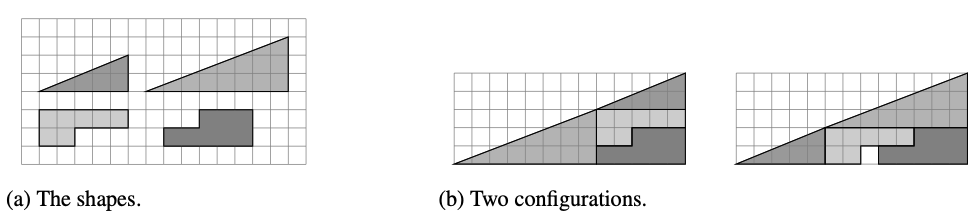
\includegraphics[width=\columnwidth]{DS2-HW2-triangles}
\caption{Figures for Question~\ref{q:triangles}}
\label{fig:triangles}
\end{center}
\end{figure}




\end{enumerate}
\end{document}